\documentclass{article} \usepackage{chtt-notes} \usepackage{stmaryrd}
\usepackage{amssymb}

\usetikzlibrary{arrows}

\scribes{Travis Hance and Paul G\"olz} \week{10}
\week{10}
% The following command will let you cross-reference labels in the
% files week1.tex, week2.tex, \ldots, week\@week.tex, where if l is a
% label in ``weekN.tex'', then you can access the label using
% \cref{WN:l}.
\doXRs

% General remark: Using \cref{label} will fill in the appropriate
% environment name. For example, ``\begin{lemma}\label{lem:foo}
%   ...\end{lemma} By \cref{lem:foo}'' will produce ``Lemma 15 ... By
% lemma~15''

\newcommand{\lift}[1]{{#1}^{\Downarrow}}
\newcommand{\meet}[1]{\bigwedge\!#1}
\newcommand{\join}[1]{\bigvee\!#1}
\newcommand{\entails}{\vdash}
\newcommand{\G}{\Gamma}
\newcommand{\atype}[1]{#1~\mathsf{type}}
\newcommand{\Nat}{\mathsf{Nat}}
\newcommand{\circled}[1]{\text{\textcircled{#1}}}
\newcommand{\tr}{\textsf{tr}}
\newcommand{\one}{\textsf{one}}
\newcommand{\zero}{\textsf{zero}}

\newcommand{\T}{\mathcal{T}}

\begin{document}
\maketitle
\section{Properties of our type system}
\marginpar{March 20, 2018}%

Last week, we formulated a mathematical account of the semantics of computational
type theory. First, we defined an operator $\T$ which operates on ``pre-type systems''
or ``candidate type systems''. 
We used the Knaster-Tarski Theorem to find the least fixed point $\tau_0$ such that
$\T(\tau_0) \subseteq \tau$.

The candidate type system $\tau$ is a collection of triples $(A, B, \varphi)$ where
$\varphi$ is a binary relation on closed values. A triple $(A, B, \varphi)$ means that
$A$ and $B$ are equal canonical types, with $\varphi$ determining the member relation
on values. Furthermore, we define
\begin{itemize}
  \item $\tau^\Downarrow(A,B,\varphi)$ iff $A \Downarrow V$, $B \Downarrow W$, and $\tau(V, W, \varphi)$.
  \item $\varphi^\Downarrow(M,N)$ iff $M \Downarrow V$, $N \Downarrow W$, and $\varphi(V,W)$.
\end{itemize}
The $\tau^\Downarrow$ and $\varphi^\Downarrow$ are essentially $\tau$ and $\varphi$ but where
we allow the arguments to be terms instead of requiring them to be values.

The operator $\T$ is defined as
\[
  \T(\tau) = \textsc{bool}(\tau) \cup \textsc{pi}(\tau) \cup \textsc{sigma}(\tau) \cup
      \textsc{eq}(\tau) \cup \textsc{nat}(\tau).
\]
$\T$ is monotone by construction. 

We'll repeat a few rules here, but they can be found in last week's notes, Section \ref{W8:subsub:tau0}.

\begin{itemize}
  \item We define \textsc{bool} as \[\textsc{bool}(-) = \{(\bool, \bool, \beta)\} \text{ where } \beta =
  \{(\true, \true), (\false, \false)\}.\]

  \item We define \textsc{nat} as \[\textsc{nat}(-) = \{(\textsf{Nat}, \textsf{Nat}, \varphi_{\textsf{Nat}})\}\] where
    $\varphi_\textsf{Nat}$ is the least fixed point containing
    \[ \{\textsc{zero}, \textsc{zero})\} \cup \{(\textsc{succ}(M), \textsc{succ}(N)) ~|~
    \varphi_\textsf{Nat}^\Downarrow(M, N) \}. \]
    Note that here we are using another induction inside the larger one. We can think of
    defining the $\textsf{Nat}$ type as a ``horizontal induction'' and defining $\tau_0$
    as a ``vertical induction.''

  \item The equality type $\Eq{A}{M}{N}$ is defined in terms of a type $A$, so the definition
      of $\textsc{eq}(\tau)$ has to be defined in terms of $\tau$.
      
      We say that $\textsc{eq}(\tau)(\Eq{A}{M}{N}, \Eq{A'}{M'}{N'}, \varphi)$ is true iff
      \begin{itemize}
      \item $\tau^\Downarrow(A, A', \varphi)$,
      \item $\varphi^\Downarrow(M,M')$ and $\varphi^\Downarrow(N,N')$,
      \item $\varphi(\textsf{refl}, \textsf{refl})$ iff $\varphi^\Downarrow(M',N)$ and
          $\varphi^\Downarrow(M,N')$.
      \end{itemize}

      Essentially, this means that $A$ and $A'$ are equal types with membership
      described by $\varphi$, and $M$ and $M'$ are equal computations according to
      $\varphi$, and same for $N$ and $N'$.

\end{itemize}

Now, $\tau_0$ is a candidate type system (by construction) but we would like to prove that
it is a real type system. To do this, we need to show it has the following properties:

\begin{enumerate}
\item \textbf{Functionality:} $\tau_0(A, B, \phi)$ and
  $\tau_0(A, B, \phi')$ imply $\phi = \phi'$
\item \textbf{\textsc{P.E.R} valued:} if $\tau_0(A, B, \phi)$, then
  $\phi$ is a partial equivalence relation
\item \textbf{Symmetry:} $\tau_0(A, B, \phi)$ implies $\tau_0(B, A, \phi)$
\item \textbf{Transitivity:} $\tau_0(A, B, \phi)$ and $\tau_0(B, C, \phi)$
  imply $\tau_0(A, C, \phi)$.
\end{enumerate}

To just give an idea of how these proofs we go, we will give a sketch of the proof
of Functionality.

\begin{theorem*}[Functionality]
Let $\tau_0$ be the least fixed point of $\T$. Then if
$\tau_0(A, B, \phi)$ and $\tau_0(A, B, \phi')$, then $\phi = \phi'$.
\end{theorem*}
\begin{proof}
  Given $\tau_0$, define another type candidate $\tau$ as
  \[ \tau(A,B,\varphi) = \forall \varphi' .~ \tau_0(A,B,\varphi') \implies \varphi = \varphi'). \]
  Essentially, this is $\tau_0$ but without the triples $(A,B,\varphi)$ where $\varphi$ is not
  unique for $A$ and $B$.

  We will show that $\T(\tau) \subseteq \tau$. This makes $\tau$ a fixed point, and since
  $\tau_0$ is the \emph{least} fixed point, we will have $\tau_0 \subseteq \tau$. Then we
  will have the desired property for $\tau_0$ as well.

  So let us show that $\T(\tau) \subseteq \tau$. Let $x \in \T(\tau)$. By definition of
  $\T$, we have either
  $x \in \textsc{bool}(\tau)$,
  $x \in \textsc{pi}(\tau)$,
  $x \in \textsc{sigma}(\tau)$,
  $x \in \textsc{eq}(\tau)$, or
  $x \in \textsc{nat}(\tau)$. We need to show that $x \in \tau$.

  We will handle two of these cases here, just to illustrate how it goes: an easier case and a harder case.
  \begin{itemize}
    \item \emph{Case} $x \in \textsc{bool}(\tau)$.

    In this case we must just have $x = (\bool, \bool, \beta)$ as defined above.
    By definition of $\tau$, we have,
    \[ \tau(\bool, \bool, \beta) = \forall \varphi' .~ \tau_0(\bool,\bool,\varphi') \implies \varphi' = \beta. \]
    But $\tau_0 = \T(\tau_0)$ and in the definition of $\T$ we can check that
    for $A=\bool$ and $B=\bool$ we must have $\varphi' = \beta$. Therefore,
    $x \in \tau$.

    This case was straightforward because $\textsc{bool}(\tau)$ does not actually depend
    on $\tau$.

    \item \emph{Case} $x \in \textsc{pi}(\tau)$.

    As a reminder, we have $\textsc{pi}(\tau)(A_0, A'_0, \rho)$ iff
    \begin{itemize}
      \item $\exists A,A',B,B'$ such that $A_0 = (x:A \to B)$ and $A'_0 = (x : A' \to B')$,
      \item $\exists \alpha$ such that $\tau(A,A',\alpha)$,
      \item $\exists \varphi$ such that $\forall M, M' .~ \alpha^\Downarrow(M,M') \implies \tau^\Downarrow([M/x]B, [M'/x]B', \varphi(M,M'))$,
      \item $\rho(M, M')$ iff
      \begin{itemize}
        \item $\exists N .~ M = \lambda x.N$,
        \item $\exists N' .~ M'= \lambda x.N'$,
        \item $\forall P, P' .~ \alpha^\Downarrow(P,P') \implies \varphi(P,P')^\Downarrow([P/x]N,[P'/x]N')$.
      \end{itemize}
    \end{itemize}
    Therefore, we have $x = (A_0, A'_0, \rho)$ where $A,A',B,B,\alpha,\varphi$ all exist as described.

    Furthermore, by definition of $\tau$, we must have that $\alpha$ and $\varphi$ are the \emph{unique}
    binary relations satisfying these properties, that is,
    \begin{itemize}
      \item $\tau_0(A,A',\alpha') \implies \alpha = \alpha'$.
      \item $\forall M,M' .~ \alpha^\Downarrow(M,M') \implies \tau_0^\Downarrow([M/x]B, [M'/x]B', \gamma) \implies \varphi(M,M') = \gamma$.
    \end{itemize}
    Furthermore, given unique $A,A',B,B',\alpha,\varphi$, the definition uniquely defines $\rho$.

    Therefore,
    \[
      \tau_0(A_0,A'_0,\rho') \implies \rho = \rho'.
    \]
    Therefore, $(A_0, A'_0, \rho) \in \tau$.
  \end{itemize}
\end{proof}

\section{Equality and transport}%

Let's revisit Intensional Type Theory (ITT).

We inductively defined the judgments,
\begin{center}
\begin{tabular}{ll}
  $\Gamma \entails M : A$ &
  $\Gamma \entails M \equiv M' : A$ \\
  $\Gamma \entails A~\textsf{type}$ &
  $\Gamma \entails A \equiv A'$ \\
  $\Gamma~\textsf{ctxt}$ &
  $\Gamma \equiv \Gamma'$
\end{tabular}
\end{center}
We also showed that if $\Gamma \entails M : A$, then $|\Gamma| \gg |M| \in |A|$, where $|\cdot|$ denotes ``erasure compilation'', i.e., removing all type lambda application and abstraction from the expression.
We also saw that $\Id{A}{M}{N}$ is not an adequate account of equality. On the plus side,
it is a partial equivalence relation and it satisfies the indiscernibility of identicals
(that is, if $\Id{A}{M}{N}$ then $M$ can be substituted for $N$.

On the negative side, there is no notion of function extensionality. $\textsf{Id}_A$ is defined
uniformly over $A$, that is, the same way for each $A$. Therefore,
we cannot possibly have
$abs \equiv id : \textsf{nat} \to \textsf{nat}$, even though we would like to,
because we must have
$abs \not\equiv id : \textsf{int} \to \textsf{int}$.

Before we can address this, we need to motivate the notion of \emph{universes}. Let's talk
more about transport and the indiscernibility of identicals. We will show that
if $\Id{A}{M}{N}$ is true then we can substitute $M$ for $N$.

\begin{theorem*}[Transport]
  Suppose $B$ is a ``predicate family''.
  \[ \Gamma, a:A \entails B~\textsf{type}. \]
  Also, suppose that $M$ is identical to $N$, with proof of identification $P$,
  \[ P : \Id{A}{M}{N}, \]
  and finally suppose that $[M/a]B$ is true,
  \[ Q : [M/a]B. \]
  Then we can substitute $N$ instead, that is we can find an element
  \[ \tr[a.B](P)(Q) : [N/a]B. \]
\end{theorem*}
\begin{proof}
  We can take
  \[
    \tr[a.B](P)(Q) = J_{a,b,\_. [a/a]B \to [b/a]B}(a.\lambda b:B . b)(Q).
  \]
\end{proof}
\begin{remark}
  By $\beta$ simplification, we can find that
  \[
    \tr[a.b](\refl{A}{M})(Q) \equiv Q : [M/a]B.
  \]
\end{remark}

Again, the only equivalence on which this works is definitional equivalence.
We could try to define a \textsf{funext} object to handle function extensions; however,
we wouldn't be able to say how \textsf{tr} or $J$ works.

Now, we will try to use $\tr$ to solve a seemingly simple problem. We want to prove that
$0 \ne 1$, or in other words, find $M$ such that
\[
  \G \entails Q : \Id{\textsf{Nat}}{\zero}{\one} \entails M : \bot.
\]
(Here, $\one$ is simply $\textsf{succ}(\zero)$.)

This should be easy; we just have to use $Q$ to substitute $\zero$ for $\one$.
For any $P$, we do have,
\[
  \G \entails Q : \tr[a.P](Q) : [\zero / a]P \to [\one / a]P.
\]
So we would be done if we could find $P$ such that $[\zero / a]P \equiv \top$ and $[\one / a]P \equiv \bot$.

Could we simply define $P$ as follow?
\[ 
  P = \textsf{NATREC}(\top; \_.\_. \bot)(a).
\]
We can't, simply because there is no such thing as \textsf{NATREC} in ITT!

In fact, one can show that there is no such $P$ in ITT. This is a problem, and we would like
to fix it. There are two possibilities.
\begin{enumerate}
\item[1.] Define a type theory with these ``large elimination forms'' (like \textsf{NATREC}) built in.
\item[2.] Allow us to just use \textsf{natrec}.
\end{enumerate}

We would like to do option 2. But this requires us to ask, what \emph{type} would the
use of \textsf{natrec} have in
$\textsf{natrec}(\top; \_.\_. \bot)(a)$ have? To answer this, we need a ``type of types,''
and this brings us to universes.
  
\section{Universes}%
\marginpar{March 22, 2018}%
To prove that zero and one are not equal, we need to be able to define a type family $P(a)$ by induction on natural numbers, which is not possible in ITT.

We might attempt to change this by adding natural recursion on the type level as a type constructor $\textsf{NATREC}$:
\[ \inferrule{\G \entails \atype{A_0} \quad \G, a: \Nat, b: \circled{?} \entails \atype{A_1} \quad \G \entails M : \Nat}{\G \entails \atype{\textsf{NATREC}(A_0; a,b.\; A_1)(M)}} \]
Even apart from the cumbersome repetition between definitions on the term and type level, it is not clear what ``type'' to give to $b$ in the premise.

What we need is a type of types, a \emph{universe} $\mathcal{U}$.
Membership in this type implies being a type:
\[ \inferrule{\G \entails A : \mathcal{U}}{\G \entails \atype{A}} \]
Then, we can do away with the distinction between terms and types, and use the usual rule for $\textsf{natrec}$ to type $P(a) \coloneqq \textsf{natrec}(\top; \_, \_. \; \bot)(a)$:
\[ \inferrule{\G \entails A_0 : \mathcal{U} \quad \G, a : \Nat, b : \mathcal{U} \entails A_1 : \mathcal{U} \quad \G \entails M : \Nat}{\G \entails \textsf{natrec}(A_0; a, b.\; A_1)(M) : \mathcal{U}} \]

To show, for example, that $P(\textsf{zero}) \equiv \top$, we lift the structural equality $P(\textsf{zero}) \equiv \top : \mathcal{U}$ using the following rule:
\[ \inferrule{\G \entails A \equiv B : \mathcal{U}}{\G \entails A \equiv B} \]

We then fill the universe with the types of ITT:
\[ \inferrule{}{\G \entails \Nat, \textsf{Bool}, \textsf{Void}, \textsf{Unit} : \mathcal{U}} \quad \quad \quad \inferrule{\G \entails A : \mathcal{U} \quad \G, a: A \entails B : \mathcal{U}}{\G \entails \Pi a : A.\; B, \Sigma a : A.\; B : \mathcal{U}}\]
\[ \inferrule{\G \entails A : \mathcal{U} \quad \G \entails M, N : A}{\G \entails \textsf{Id}_A(M, N) : \mathcal{U}} \]
And so forth.

Ideally, we would like $\mathcal{U}$ to encode all types.
However, we cannot set $\mathcal{U} : \mathcal{U}$ because this would be inconsistent by Russel's paradox.
To solve this problem, we define not just a single universe $\mathcal{U}$, but an infinite hierarchy of universes $\mathcal{U}_0: \mathcal{U}_1: \mathcal{U}_2 \dots$.
Every universe is maximal in the sense that it is closed under our type constructors by the aforem-entioned rules.
This hierarchy is cumulative as per the following rule:
\[ \inferrule{\G \entails M : \mathcal{U}_i}{\G \entails M : \mathcal{U}_{i + 1}}\]

It is worth pointing out that our types can now include arbitrarily complicated computation.

\section{Higher identification}
If $\textsf{Id}_A$ should be a notion of equality, we would expect for example $\textsf{Id}_{\Nat \to \Nat}(f, g)$ to be inhabited iff $\Pi a: \Nat.\; \textsf{Id}_{\Nat}(f~a, g~a)$ is.

Now that we introduced universes, what should $\textsf{Id}_{\mathcal{U}}$ look like?
It would be natural to consider two types $A, B : \mathcal{U}$ as equal iff they are isomorphic, i.e., if there are functions $f : A \to B$ and $g : B \to A$ such that $g \circ f \circled{=} \textit{id}$ and $f \circ g \circled{=} \textit{id}$.
But which relation should we use for ``$\circled{=}$''?
Requiring structural equality as $g(f(a)) \equiv a$ is way to fine.
A better idea would be to require $\textsf{Id}_A(g(f(a)), a)$, and Vladimir Voevodsky's univalence goes into that direction. \medskip

In \cref{W7:sec:identitytypes} of Week~7, we considered different ways of constructing elements of identity types:
\begin{itemize}
    \item $\textsf{refl}_A(M) : \textsf{Id}_A (M, M)$. Leaving the type implicit, we suggestively set $\textit{id} \coloneqq \textsf{refl}_A(M)$.
        We illustrate this as follows:
        \begin{center}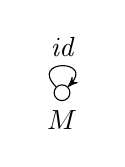
\begin{tikzpicture}[->,>=stealth',auto,node distance=2cm,every loop/.style={min distance=5mm,in=45,out=135,looseness=5}]
\node [circle, draw=black, inner sep=0pt, minimum size=2mm] (a) [label=below:$M$] {};
        \path[->] (a) edge  [loop above] node {$\textit{id}$} ();\end{tikzpicture}\end{center}
    \item $\textsf{sym}_A(P) : \textsf{Id}_A (N, M)$ for $P : \textsf{Id}_A(M, N)$. Set $P^{-1} \coloneqq \textsf{sym}_A(P)$.
        \begin{center}\begin{tikzpicture}[->,>=stealth',auto,node distance=2cm,every loop/.style={min distance=5mm,in=45,out=135,looseness=5}]
\node [circle, draw=black, inner sep=0pt, minimum size=2mm] (a) [label=below:$M$] {};
\node [circle, draw=black, inner sep=0pt, minimum size=2mm] (b) [right=of a,label=below:$N$] {};
\draw [->, bend left] (a) to node [above] {$P$} (b);
        \draw [->, bend left] (b) to node [below] {$P^{-1}$} (a);\end{tikzpicture}\end{center}
    \item $\textsf{trans}_A(Q, R) : \textsf{Id}_A(M, P)$ for $Q : \textsf{Id}_A(M, N)$ and $R : \textsf{Id}_A(N, P)$. Denote this by $Q \circ R$.
        \begin{center}\begin{tikzpicture}[->,>=stealth',auto,node distance=2cm,every loop/.style={min distance=5mm,in=45,out=135,looseness=5}]
\node [circle, draw=black, inner sep=0pt, minimum size=2mm] (a) [label=below:$M$] {};
\node [circle, draw=black, inner sep=0pt, minimum size=2mm] (b) [right=of a,label=below:$N$] {};
\node [circle, draw=black, inner sep=0pt, minimum size=2mm] (c) [right=of b,label=below:$P$] {};
\draw [->] (a) to node [above] {$Q$} (b);
\draw [->] (b) to node [above] {$R$} (c);
        \draw [->, bend right] (a) to node [below] {$Q \circ R$} (c);\end{tikzpicture}\end{center}
\end{itemize}

We would expect this structure to respect the groupoid\footnote{A groupoid is a generalization of a group in which elements are ``typed.'' Here, we can only concatenate paths $P$ and $Q$ as $P \circ Q$ if $P : \textsf{Id}_A(M, N)$ and $Q : \textsf{Id}_A(N, P)$, i.e., if the endpoint of path $P$ equals the starting point of path $Q$.} laws:
\begin{enumerate}
    \item \label{idrev} $\mathit{id}^{-1} \circled{=} \mathit{id}$
    \item \label{trid} $Q \circ \mathit{id} \circled{=} Q$
    \item \label{idtr} $\mathit{id} \circ R \circled{=} R$
    \item $P^{-1} \circ P \circled{=} \mathit{id}$
    \item \label{pinvid} $P \circ P^{-1} \circled{=} \mathit{id}$
    \item \label{assoc} $P \circ (Q \circ R) \circled{=} (P \circ Q) \circ R$
    \item $(P^{-1})^{-1} \circled{=} P$
\end{enumerate}
As we discussed in Week~7, choosing ``$\equiv$'' for ``$\circled{=}$'' only satisfies some of these laws.
For example, property~\ref{idrev} is true, whereas at most one out of properties~\ref{trid} and \ref{idtr} holds, depending on the exact program used to implement transitivity.

To get the groupoid structure, we instead choose $\textsf{Id}_{\textsf{Id}_A}$ for ``$\circled{=}$'':

For instance, consider Law~\ref{pinvid}:
Suppose that we have $P : \textsf{Id}_A(M, N)$ and thus $P^{-1} : \textsf{Id}_A(n, M)$.
Then, by using $\mathit{id}^{-1} \equiv \mathit{id}$ and $\mathit{id} \circ \mathit{id} \equiv \mathit{id}$, one verifies that
\[J_{a,\_,p.\; \textsf{Id}_{\textsf{Id}_A(a,a)}(p \circ p^{-1}, \textsf{refl}_A(a))}(a.\; \textsf{refl}_{\textsf{Id}_A(a,a)}(\textsf{refl}_A(a)))(P) : \textsf{Id}_{\textsf{Id}_A(M, M)}(P \circ P^{-1}, \textsf{refl}_A(M)).\]

Or consider Law~\ref{assoc}:
\begin{center}\begin{tikzpicture}[->,>=stealth',auto,node distance=2cm,every loop/.style={min distance=5mm,in=45,out=135,looseness=5}]
\node [circle, draw=black, inner sep=0pt, minimum size=2mm] (a) [label=below:$S$] {};
\node [circle, draw=black, inner sep=0pt, minimum size=2mm] (b) [right=of a] {};
\node [circle, draw=black, inner sep=0pt, minimum size=2mm] (c) [right=of b] {};
\node [circle, draw=black, inner sep=0pt, minimum size=2mm] (d) [right=of c,label=below:$F$] {};
\draw [->] (a) to node [above] {$P$} (b);
\draw [->] (b) to node [above] {$Q$} (c);
\draw [->] (c) to node [above] {$R$} (d);
\draw [->, bend left] (a) to node [above] {$P \circ Q$} (c);
\draw [->, bend right] (b) to node [below] {$Q \circ R$} (d);
\draw [->, out=50, in=130] (a) to node [above] {$(P \circ Q) \circ R$} (d);
\draw [->, out=-50, in=-130] (a) to node [below] {$P \circ (Q \circ R)$} (d);\end{tikzpicture}\end{center}
Again, given $P, Q, R$, we can find a term of type $\textsf{Id}_{\textsf{Id}_A(S, F)}((P \circ Q) \circ R, P \circ (Q \circ R))$.
Borrowing intuitions from homotopy theory, this term can be thought of as a continuous deformation (a \emph{homotopy}) of the path corresponding to $(P \circ Q) \circ R$ into the path corresponding to $P \circ (Q \circ R)$.

Generally, the groupoid laws hold ``up to higher identification''.
We call the nesting depth of $\textsf{Id}_{\textsf{Id}_{._{._{.}}}}$ its dimension.
Again, in the language of homotopy theory, this corresponds to going from points (dimension 0) to paths between points (dimension 1) to paths between paths between points (dimension 2) and so forth.
Since the groupoid laws for objects of some dimension hold up to an equivalence of one higher dimension, the iterated $\textsf{Id}$s form a so-called \emph{$\infty$-groupoid}.

\section{Outlook}
When is $f : A \to B$ a bijection?
One way of defining this is the following:
For every element $b : B$, call its preimages $f^{-1}(b) \coloneqq \Sigma a: A. \; \textsf{Id}_{B}(f(a), b)$ its \emph{homotopy fiber}.
$f$ is a bijection iff every fiber contains exactly one element.
Equivalently, we might require that every fiber contains a \emph{center of contraction} $c$ such that, for every element $c'$ of the fiber, there is a ``path from $c$ to $c'$'', i.e., a term of type $\textsf{Id}_A(c, c')$.
In this case, we say that the fibers are contractible.

Next week, we will study the univalence axiom, which is based on this idea.

\bibliographystyle{plainnat} \bibliography{ctt}

\end{document}

%%% Local Variables:
%%% mode: latex
%%% TeX-master: t
%%% End:
